\documentclass[12pt, titlepage]{article}

\usepackage{fullpage}
\usepackage[round]{natbib}
\usepackage{multirow}
\usepackage{booktabs}
\usepackage{tabularx}
\usepackage{graphicx}
\usepackage{float}
\usepackage{hyperref}
\hypersetup{
    colorlinks,
    citecolor=blue,
    filecolor=black,
    linkcolor=red,
    urlcolor=blue
}

%% Comments

\usepackage{color}

\newif\ifcomments\commentstrue %displays comments
%\newif\ifcomments\commentsfalse %so that comments do not display

\ifcomments
\newcommand{\authornote}[3]{\textcolor{#1}{[#3 ---#2]}}
\newcommand{\todo}[1]{\textcolor{red}{[TODO: #1]}}
\else
\newcommand{\authornote}[3]{}
\newcommand{\todo}[1]{}
\fi

\newcommand{\wss}[1]{\authornote{blue}{SS}{#1}} 
\newcommand{\plt}[1]{\authornote{magenta}{TPLT}{#1}} %For explanation of the template
\newcommand{\an}[1]{\authornote{cyan}{Author}{#1}}

%% Common Parts

\newcommand{\progname}{Mechtronics Enigeering} % PUT YOUR PROGRAM NAME HERE
\newcommand{\authname}{Team 32, Wingman
\\ Edward He
\\ Erping Zhang
\\ Guangwei Tang
\\ Peng Cui
\\ Peihua Jin } % AUTHOR NAMES                  

\usepackage{hyperref}
    \hypersetup{colorlinks=true, linkcolor=blue, citecolor=blue, filecolor=blue,
                urlcolor=blue, unicode=false}
    \urlstyle{same}
                                


\newcounter{acnum}
\newcommand{\actheacnum}{AC\theacnum}
\newcommand{\acref}[1]{AC\ref{#1}}

\newcounter{ucnum}
\newcommand{\uctheucnum}{UC\theucnum}
\newcommand{\uref}[1]{UC\ref{#1}}

\newcounter{mnum}
\newcommand{\mthemnum}{M\themnum}
\newcommand{\mref}[1]{M\ref{#1}}

\begin{document}

\title{System Design for \progname{}} 
\author{\authname}
\date{\today}

\maketitle

\pagenumbering{roman}

\section{Revision History}

\begin{tabularx}{\textwidth}{p{3cm}p{2cm}X}
\toprule {\bf Date} & {\bf Version} & {\bf Notes}\\
\midrule
Date 1 & 1.0 & Notes\\
Date 2 & 1.1 & Notes\\
\bottomrule
\end{tabularx}

\newpage

\section{Reference Material}

This section records information for easy reference.

\subsection{Abbreviations and Acronyms}

\renewcommand{\arraystretch}{1.2}
\begin{tabular}{l l} 
  \toprule		
  \textbf{symbol} & \textbf{description}\\
  \midrule 
  \progname & Explanation of program name\\
  \wss{...} & \wss{...}\\
  \bottomrule
\end{tabular}\\

\newpage

\tableofcontents

\newpage

\listoftables

\listoffigures

\newpage

\pagenumbering{arabic}


\section{Purpose}

This Document mainly talks about the design of the project, including the behavior, variables and interfaces used in the design. It will also talk about the design of the hardware component of the object, with some electrical components used and some communication protocols in the design.

\section{Scope}

The system will be designed to track the movement of the object to get the latest location information about it so that the user can always get the desired output. The user will be able to login and start the program through their own username and password. Then the information about the object will be detected through some image processing algorithms and will be stored into certain files. The user can locate desired objects through the searching interface by providing several searching keys. 


\subsection{Context Diagram}

The following pictures shows the design of the context diagram of the project. In this diagram, the user can interact with the SmartVault by logging in and provide key information about the object and SmartVault will output searching results to the user. There will be a camera located in the room that will keep sending images to SmartVault used for image processing. The motor will interact with SmartVault so to change the angular position of the camera. SmartVault will send or update information stored in the database. It will also extract desired information from the database. 

\begin{figure}[H]
    \centering
    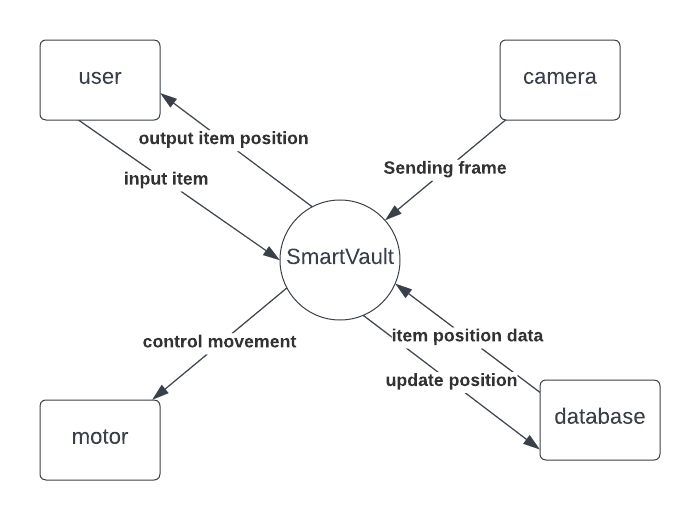
\includegraphics[scale=0.8]{work_context.png}
    \caption{The Picture of Use Case Diagram}
\end{figure}

\section{Project Overview}
The purpose of this project is to create a system that help the user to locate their belongs in a certain space. SmartVault will allow user to login and start the camera, by detecting the movement of the object dynamically, it will keep recording and updating positional information about the objects that are detected in the camera. Then user can detect the position of the object by sorting through the database with certain searching information.
\subsection{Normal Behaviour}
SmartVault will start operating once the user login successfully and provide technical support when the user needs. It will store the position information of objects in the database for further use. The movement of the camera is controlled by the motor so that the monitoring angle will always in best angle. It will automatically detect the movement of object using image processing method. THIS LINE IS USED FOR OTHER MOCULE. TALKS ABOUT THE REST OF DEFINITION OF HARDWARE PART. To achieve different behaviors, different components are describes in the table below with their purpose. 

\begin{table}[H]
\begin{center}
\caption {The Table of Division of Components and Purpose}
    \begin{tabular}{| p{5cm}| p{9.5cm} |}
    \hline
    \textbf{Component Name} & \textbf{Component Purpose}  \\
    \hline
    Login & Manage login information and Technical Support Information \\
    \hline
    Database  & Stores the position information of object detected inside the room\\
    \hline
    Image Process & Identifies movement of object and takes screen shot\\
    \hline
    Motor & Control the angle of the camera monitoring the room\\
    \hline
    Description & As part of the project hard requirement for Mechatronics group, the design can not be all software based \\
    \hline
    \end{tabular}
\end{center}
\end{table}
\subsection{Undesired Event Handling}

\wss{How you will approach undesired events}

\subsection{Component Diagram}
The picture shown below presents different components known as modules in this project. All the modules are divided into two big module group: Software Module and Hardware Module. 

\begin{figure}[H]
    \centering
    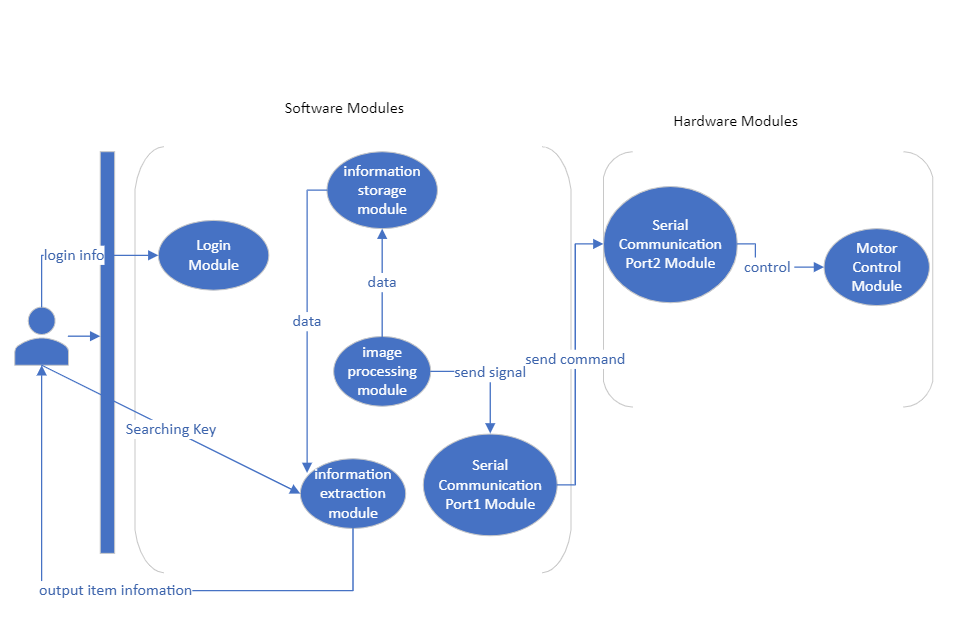
\includegraphics[scale=0.3]{Module.png}
    \caption{The Picture of Component Diagram}
\end{figure}

\subsection{Connection Between Requirements and Design} \label{SecConnection}

To achieve the requirements mentioned in Software Requirement Specification Document, some specific designs are made and described in the table shown below. 

\begin{table}[H]
\begin{center}
\caption {The Table of Connection Between Requirements and Design}
    \begin{tabular}{| p{8cm}| p{7cm} |}
    \hline
    \textbf{Design Actions} & \textbf{Requirements}  \\
    \hline
    Image Processing Method & IPR1, IPR2, IPR3, IPR4,  \\
    \hline
    Database  & IPR5, IPR6, IPR7, IPR8, IPR9, RFR1, CAR1, LOR1\\
    \hline
    Customization Button & UIR1, UIR2\\
    \hline
    Vedio shown in the window & UIR4\\
    \hline
    Protection Cover & APR1, APR2 \\
    \hline
    Text Prompt & EUR2, LER1, LER2, RFR2\\
    \hline
    Visualized Window & EUR2, UPR1, ACR1\\
    \hline
    Setting Username and Password & SCR2, AER1, INR1, INR2, PRR1, PRR2, CPR1\\
    \hline
    Technical Support Window & MAR1\\
    \hline
    Motor Communication Protocol & SCR3, RAR1\\
    \hline
    \end{tabular}
\end{center}
\end{table}

\section{System Variables}

\wss{Include this section for Mechatronics projects}

\subsection{Monitored Variables}

\subsection{Controlled Variables}

\subsection{Constants Variables}

\section{User Interfaces}

Two user interfaces will be used for this project, one is for the user to login and the other is used for searching the position information of the desired object. This section will mainly talks about these two interfaces in the following paragraphs. 

\subsection{Login Interface}
The Login Interface is used to show let the user start the program. It will also provide the contact information of the technical support. The picture shown below describes the FSM of the Login Interface. When the user starts the program ans enters correct username and password, the original window quits and comes up with the Search Window. If the user enters wrong username or passsword, the wondown will not change and asks the user to retry. If the user want to get the technical support, the Technical Support will come up. 

\begin{figure}[H]
    \centering
    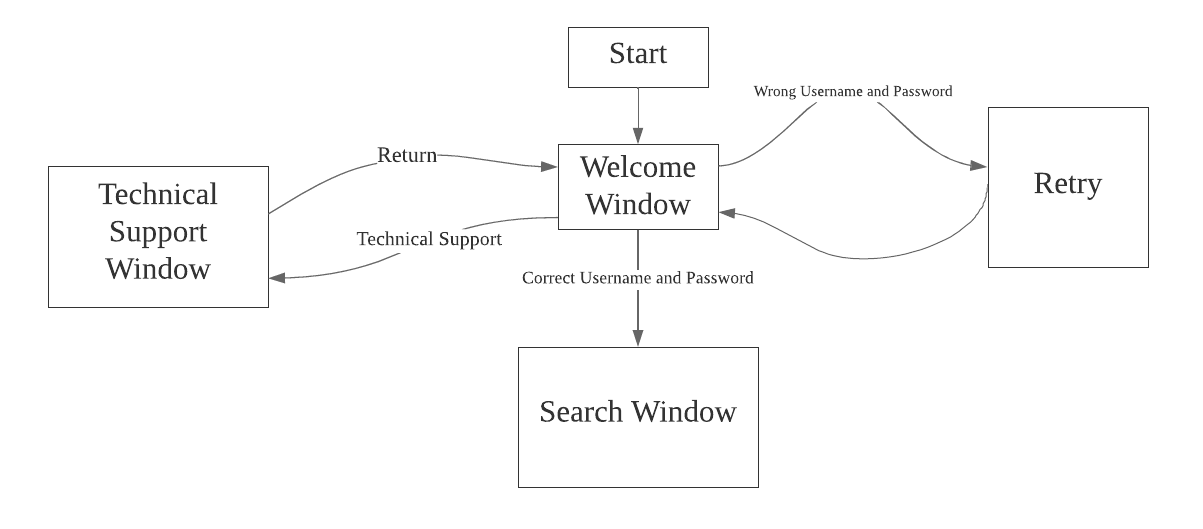
\includegraphics[scale=0.8]{FSM1.png}
    \caption{The Design of Welcome Window}
\end{figure}

WHen it comes to the Design of Window, the first one is the Welcome Window. The Welcome Window asks the user to input the username and password. If the user enters correct username and password, the window is closed and the Confirmation Windown will come up, which will be described in the paragraphs below. The Technical Support Window gives the emails of each team member. The Design of Welcome and Technical Support Window is shown in the pictures below. 

\begin{figure}[H]
    \centering
    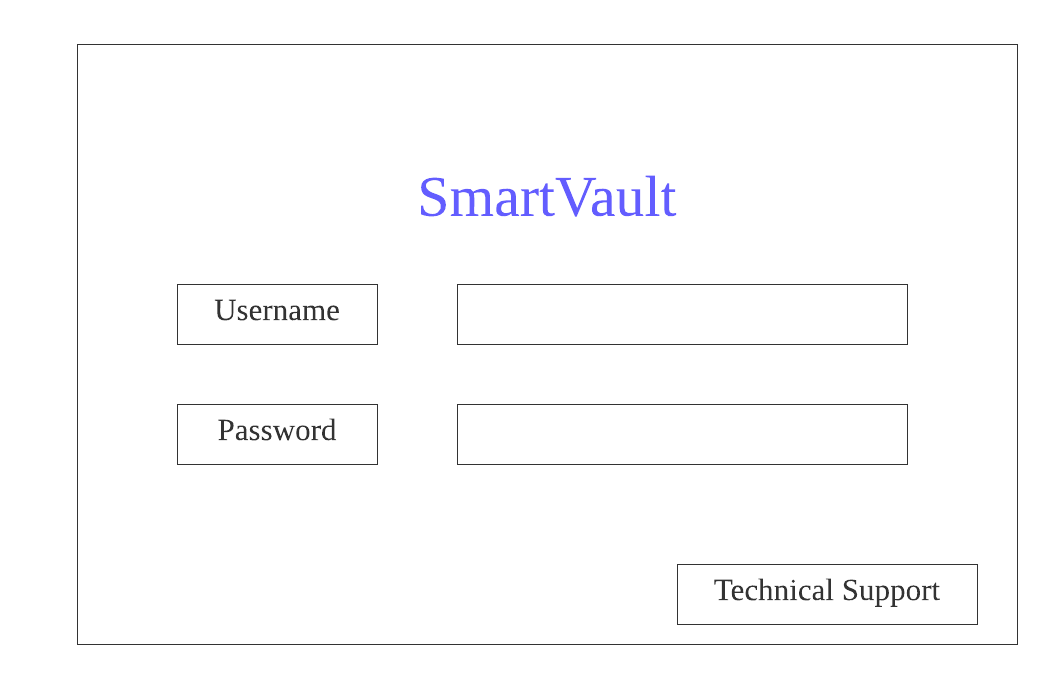
\includegraphics[scale=0.8]{Welcome.png}
    \caption{The Design of Welcome Window}
\end{figure}

\begin{figure}[H]
    \centering
    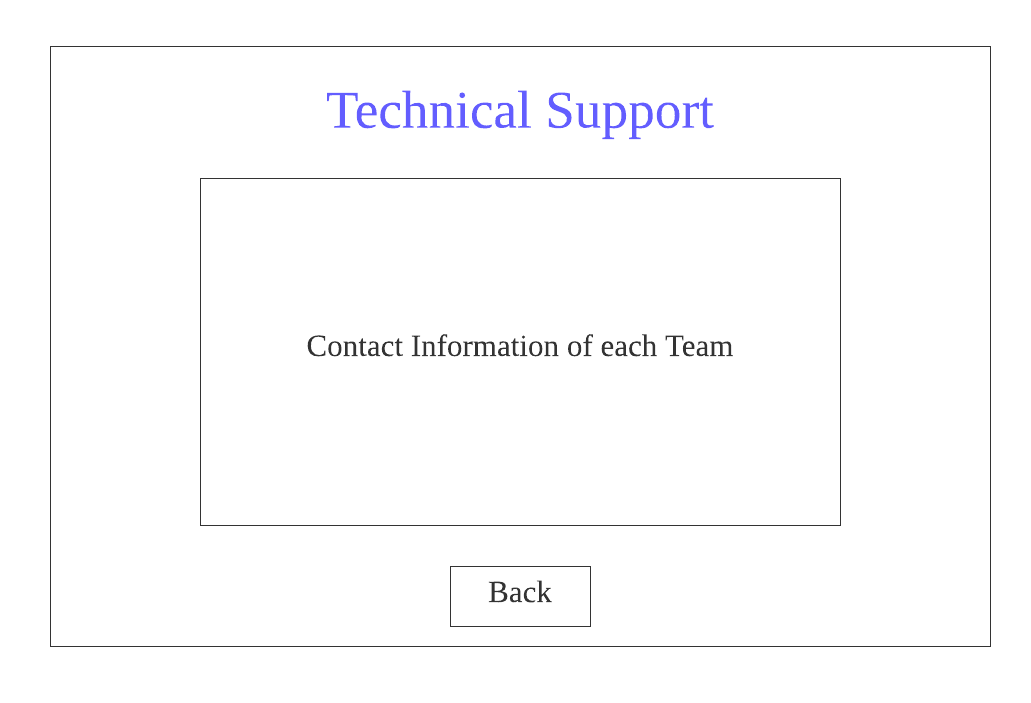
\includegraphics[scale=0.8]{Technical.png}
    \caption{The Design of Technical Support Window}
\end{figure}

\subsection{Searching Interface}

The Searching Interface is used to help the user to locate the position of the object. The picture shown below describe the FSM of the project. After the program starts, the image processing method will be used to record initial condition of the object detected in the roon through the image taken by the camera. The program will wait for further changes. The motor will rotate the camera if the user detected is not in the certer of the camera or certain percentage of area of the images is blocked. When the movement of an object is detected, if it is moved by human, the program will track the movement of hands and update the information stored in the database. If it is moved by other objects, the program will only update it final state. The data base willl only record the object that moves in the area. When the user want to search certain object, the program will allow the user to input some information about the object like the approximate time. Then a list of pictures meets the information will be provided and wait for the user to choose. If the desired object is within the list and the user has confirmed it, the algorithm will finish. If the object is not found, the initial pictures will be pulled out and let the user to choose. The object is marked "Taken out" if the object is still not found. 

\begin{figure}[H]
    \centering
    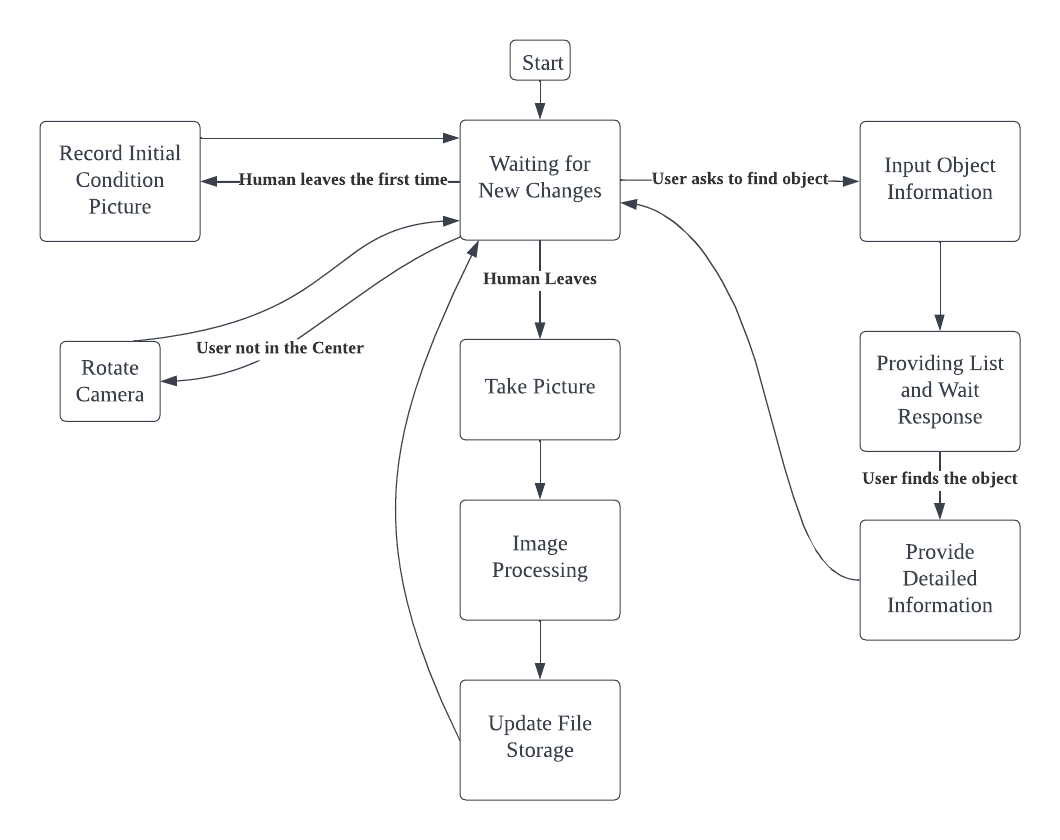
\includegraphics[scale=0.8]{FSM.png}
    \caption{The Finite State Machine of Searching Interface}
\end{figure}

For the searching interface of this project, the window will come up after the use has successfully logging into the system. A simple design of that interface is shown in the figure below. On the left hand side the images taken by the camera will be shown. On the right hand side, the object-searching algorithm will be used. If the user want to search for one desired object, the system will ask the user to input several informations about that object. After user has finished entering the information and press search, a new window will appear. It will provide several pictures that meets the input information. After the user has confirmed the final result, the result window will come up with the information that the user needs about the object.
If the user press "Object not Found ?" button, another confirmation window with the same payttern will come up but with pictures that present the initial condition. An error window is designed to tell the user that the object may be taken out by human. It will aso leave a button to return to the Searching Window. 

\begin{figure}[H]
    \centering
    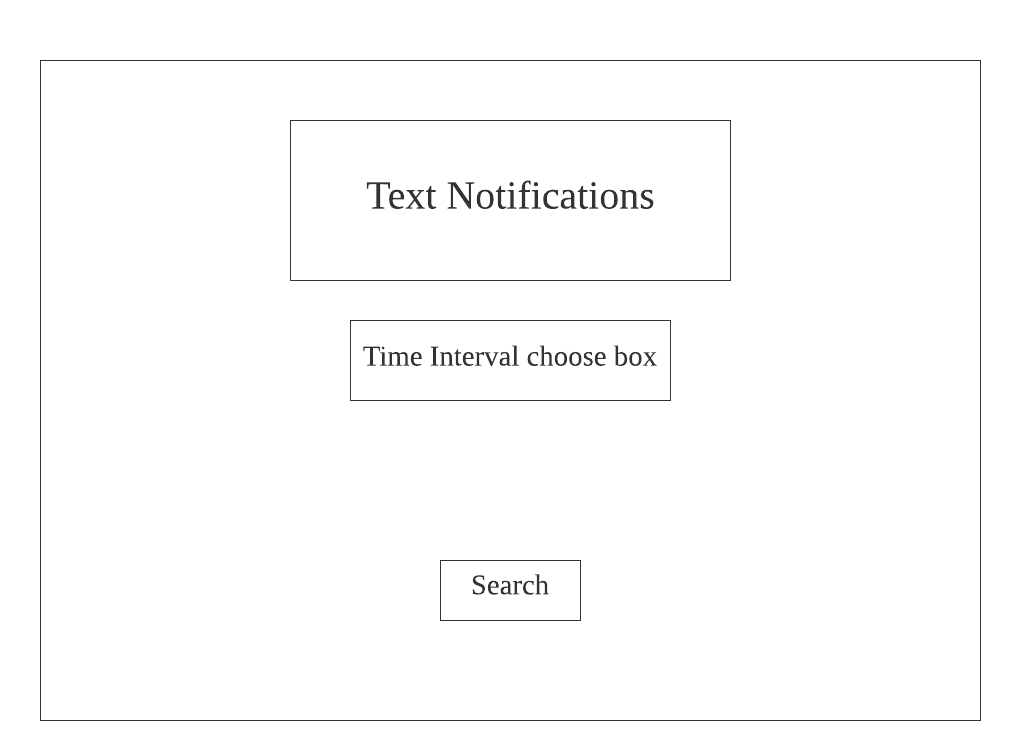
\includegraphics[scale=0.6]{Search.png}
    \caption{The Design of Searching Window}
\end{figure}

\begin{figure}[H]
    \centering
    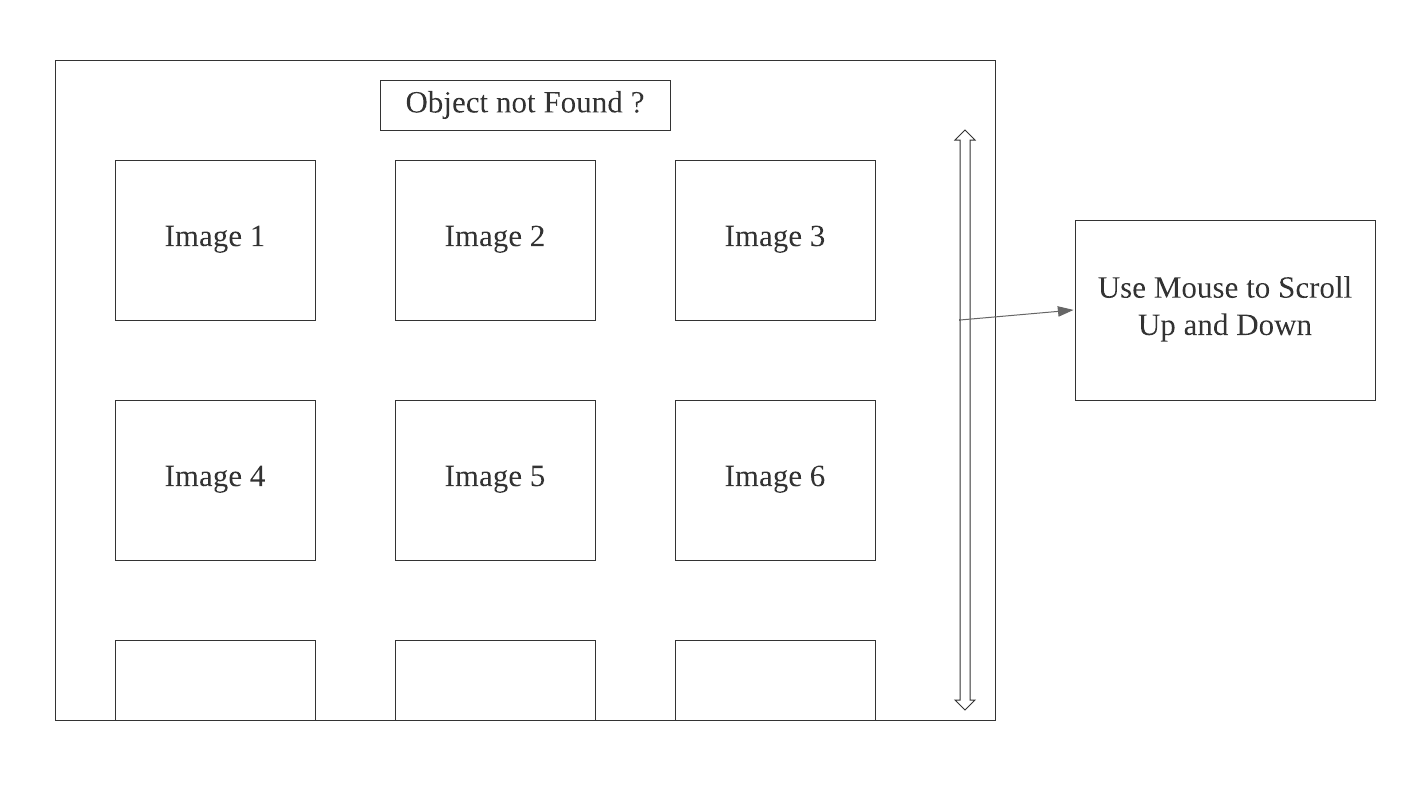
\includegraphics[scale=0.6]{Confirmation.png}
    \caption{The Design of Confirmation Window}
\end{figure}

\begin{figure}[H]
    \centering
    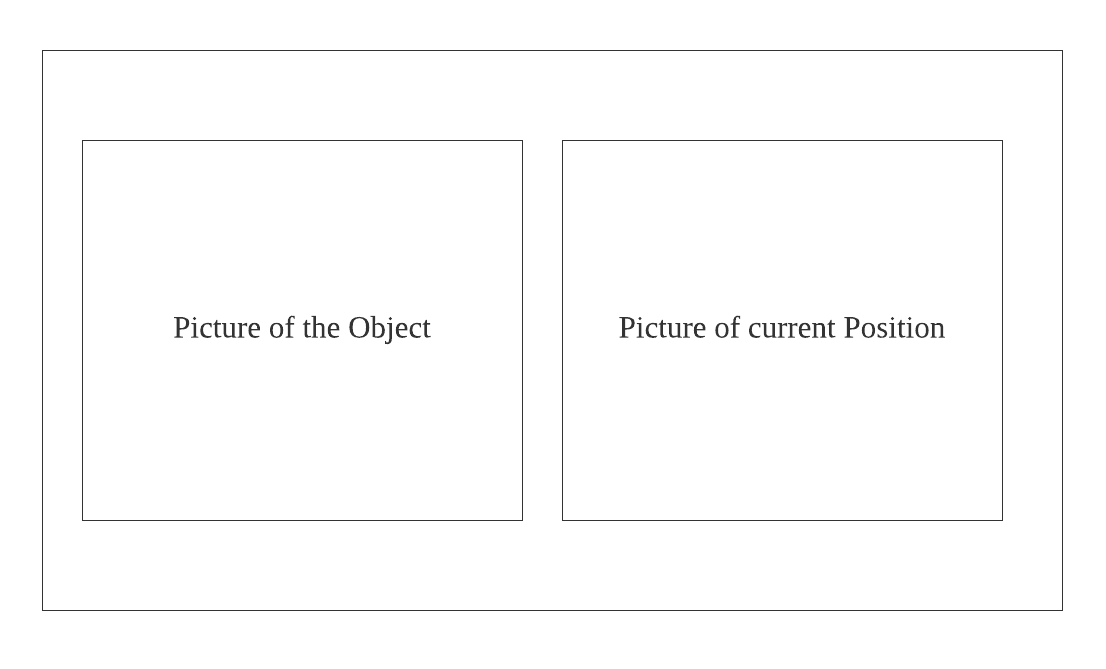
\includegraphics[scale=0.6]{Output.png}
    \caption{The Design of Output Window}
\end{figure}

\begin{figure}[H]
    \centering
    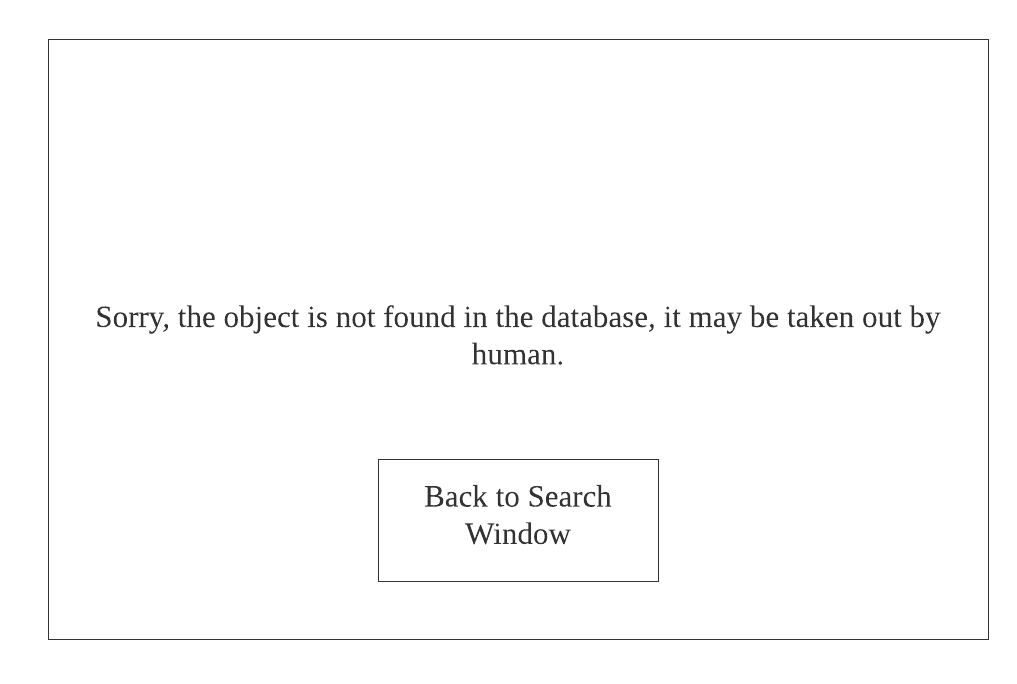
\includegraphics[scale=0.6]{Error.png}
    \caption{The Design of Error Window}
\end{figure}

\section{Design of Hardware}

\wss{Most relevant for mechatronics projects}
\wss{Show what will be acquired}
\wss{Show what will be built, with detail on fabrication and materials}
\wss{Include appendices as appropriate, possibly with sketches, drawings, CAD, etc}

\section{Design of Electrical Components}

\wss{Most relevant for mechatronics projects}
\wss{Show what will be acquired}
\wss{Show what will be built, with detail on fabrication and materials}
\wss{Include appendices as appropriate, possibly with sketches, drawings,
circuit diagrams, etc}

\section{Design of Communication Protocols}

\wss{If appropriate}

\section{Timeline}

\wss{Schedule of tasks and who is responsible}

% \bibliographystyle {plainnat}
% \bibliography{../../../refs/References}

\newpage{}

\appendix

\section{Interface}

\wss{Include additional information related to the appearance of, and
interaction with, the user interface}

\section{Mechanical Hardware}

\section{Electrical Components}

\section{Communication Protocols}

\section{Reflection}

The information in this section will be used to evaluate the team members on the
graduate attribute of Problem Analysis and Design.  Please answer the following questions:

\begin{enumerate}
  \item What are the limitations of your solution?  Put another way, given
  unlimited resources, what could you do to make the project better? (LO\_ProbSolutions)
  \item Give a brief overview of other design solutions you considered.  What
  are the benefits and tradeoffs of those other designs compared with the chosen
  design?  From all the potential options, why did you select documented design?
  (LO\_Explores)
\end{enumerate}

\end{document}
